\documentclass[10pt]{article}
\usepackage{tmlr}
% If accepted, instead use the following line for the camera-ready submission:
%\usepackage[accepted]{tmlr}
% To de-anonymize and remove mentions to TMLR, for example for posting to preprint
% servers, instead use:
%\usepackage[preprint]{tmlr}

\usepackage{booktabs}
\usepackage{graphicx}
\usepackage{hyperref}
\usepackage{url}

\graphicspath{{../figures/}}

\title{Confidence Without Competence: Calibration Risks in Real-World LLM Deployment Pipelines}

% Keep author information anonymous for review. Replace this block only for
% accepted or preprint versions.
\author{\name Anonymous Authors}

\newcommand{\ptq}{\textsc{PTQ}}
\newcommand{\qlora}{\textsc{QLoRA}}
\newcommand{\ece}{\textsc{ECE}}
\newcommand{\nll}{\textsc{NLL}}

\def\month{MM}
\def\year{YYYY}
\def\openreview{\url{https://openreview.net/forum?id=XXXX}}

\begin{document}

\maketitle

\begin{abstract}
The deployment of large language models (LLMs) in production systems increasingly relies on model compression techniques to meet resource constraints. Two dominant pipelines have emerged: post-training quantization (\ptq), which applies quantization to a pretrained and instruction-tuned model, and \qlora, which fine-tunes low-rank adapters in a quantized weight space. While prior work compares these pipelines on task accuracy, their effect on confidence calibration, the alignment between a model's stated confidence and its actual accuracy, remains understudied. Poor calibration poses a direct safety risk in production agents: a model that is confidently wrong is more dangerous than one that is correctly uncertain. In this work, we empirically compare the calibration behavior of both deployment pipelines using Gemma-2-2B as the base model. We evaluate across MMLU, ARC-Challenge, and TruthfulQA using Expected Calibration Error (\ece), Brier score, Negative Log-Likelihood (\nll), and behavioral metrics including overconfidence rate. We find that the evaluated \ptq pipeline exhibits an overconfidence rate of 29.7\% and \ece{} of 0.293, compared with 0.9\% and 0.038 for the \qlora{} pipeline, a 7.7x calibration gap despite the \ptq{} pipeline achieving 23 percentage points higher task accuracy. However, this comparison is confounded by differences in instruction-tuning scale. We argue that accuracy alone is an insufficient criterion for deployment decisions when calibration safety is at stake.
\end{abstract}

\section{Introduction}

The deployment of language models at scale has accelerated the adoption of quantization as a standard compression technique. Four-bit quantized models have become common for local and edge deployment because they enable inference on consumer hardware at the cost of some precision. Two deployment paradigms dominate. In post-training quantization (\ptq), a professionally instruction-tuned model is quantized after training. In \qlora-based deployment, a base model is quantized first and then fine-tuned through low-rank adapters on task-specific data \citep{dettmers2023qlora,hu2022lora}.

Practitioners currently choose between these pipelines based primarily on two criteria: task accuracy and inference speed. A critical dimension is often overlooked: confidence calibration. A model is well calibrated if its stated confidence on a prediction correlates with the probability that the prediction is correct. A model with 80\% confidence on a set of questions should answer approximately 80\% of them correctly. Miscalibration, particularly overconfidence, is a known failure mode in deployed AI systems, leading to hallucinated facts stated with high certainty, inappropriate downstream decisions by systems relying on model confidence scores, and erosion of user trust \citep{guo2017calibration,kadavath2022know}.

This paper presents an empirical study comparing the calibration behavior of \ptq{} and \qlora{} deployment pipelines on standard NLP benchmarks. We make the following contributions:
\begin{itemize}
    \item We evaluate calibration across two real-world deployment pipelines using a controlled base model family, Gemma-2-2B \citep{gemma2024}, measuring \ece, Brier score, \nll, and overconfidence rate.
    \item We find a consistent 7.7x \ece{} gap and 33x overconfidence gap in favor of \qlora{} across all three benchmarks, despite the \ptq{} pipeline achieving higher task accuracy.
    \item We discuss the mechanistic implications and identify the confound between pipeline choice and instruction-tuning scale as a direction for future controlled ablation.
\end{itemize}

Our findings suggest that the \ptq{} deployment pipeline, as currently practiced in our evaluation setting, is associated with systematically higher overconfidence. This may represent a safety risk for production agents, particularly in domains requiring reliable uncertainty quantification.

To support reproducibility, we will release all code, configurations, and evaluation scripts. An anonymized artifact can be provided during review.

\section{Related Work}

\subsection{Confidence calibration in neural networks}

\citet{guo2017calibration} showed that modern neural networks are often poorly calibrated, tending to produce overconfident predictions despite high accuracy. They popularized Expected Calibration Error as a metric for measuring this mismatch and demonstrated that temperature scaling, a simple post-hoc adjustment, can significantly improve calibration. A key takeaway from their work is that predictive accuracy and calibration are not inherently correlated, motivating evaluation settings where models with differing accuracies are compared in terms of confidence reliability.

LLM-specific work has also examined whether models know what they know. \citet{kadavath2022know} found that models can partially predict their own correctness, but still struggle with calibration under distributional and task shifts. This motivates direct calibration evaluation rather than relying on task accuracy alone.

\subsection{Quantization and \qlora}

\citet{dettmers2023qlora} introduced \qlora{} and 4-bit NormalFloat (NF4) quantization, enabling efficient low-rank fine-tuning of quantized LLMs while preserving much of the performance of full-precision fine-tuning. Their evaluation primarily focused on accuracy and resource efficiency, not calibration properties. We also use an 8-bit optimizer from the bitsandbytes ecosystem, following prior work on memory-efficient quantized optimization \citep{dettmers2022optimizers}.

Post-training quantization methods for large language models have also been explored extensively. Techniques such as GPTQ \citep{frantar2023gptq} and AWQ \citep{lin2024awq} improve quantization fidelity and efficiency, typically optimizing for accuracy and inference speed. However, the impact of these methods on model calibration remains comparatively understudied.

\subsection{Calibration and safety}

Calibration has important implications for AI safety, particularly in domains where model confidence informs downstream decisions. Overconfident incorrect predictions can be especially problematic in settings such as medical decision-making, autonomous systems, and agent-based workflows.

The TruthfulQA benchmark \citep{lin2022truthfulqa} was designed to evaluate whether language models produce answers that are not only plausible but factually correct, particularly in the presence of common misconceptions. While not a direct calibration metric, it is relevant to calibration-focused analyses because it tests the tendency of models to produce incorrect but plausible answers.

\section{Methodology}

\subsection{Pipeline definitions}

We compare two deployment pipelines that reflect current real-world practice:

\paragraph{Pipeline A (\ptq).}
We load \texttt{google/gemma-2-2b-it}, Google's instruction-tuned variant of Gemma-2-2B, with 4-bit NF4 quantization applied at inference time via bitsandbytes. This model was trained in full precision on Google's instruction-following data and subsequently quantized. This represents the \ptq{} deployment paradigm: fine-tune in high precision, then compress for deployment.

\paragraph{Pipeline B (\qlora).}
We load \texttt{google/gemma-2-2b}, the base model, with 4-bit NF4 quantization; apply LoRA adapters with rank $r=16$ and $\alpha=32$ to all attention projection matrices \texttt{q\_proj}, \texttt{k\_proj}, \texttt{v\_proj}, and \texttt{o\_proj}; and fine-tune on 800 samples from the Alpaca instruction-following dataset \citep{taori2023alpaca} for two epochs using paged AdamW 8-bit optimization. This represents the \qlora{} paradigm: quantize first, then fine-tune through the quantized weight space. Table~\ref{tab:pipeline-comparison} summarizes the experimental differences between the two pipelines.

\begin{table}[t]
\caption{Pipeline comparison. Both pipelines use the same Gemma-2-2B model lineage and the same NF4 4-bit quantization format.}
\label{tab:pipeline-comparison}
\begin{center}
\begin{tabular}{lll}
\toprule
Property & Pipeline A (\ptq) & Pipeline B (\qlora) \\
\midrule
Base model & \texttt{google/gemma-2-2b-it} & \texttt{google/gemma-2-2b} \\
Instruction tuning & Google, full precision, large scale & Custom \qlora, 800 Alpaca samples \\
Quantization timing & After instruction tuning & Before instruction tuning \\
Quantization format & NF4 4-bit via bitsandbytes & NF4 4-bit via bitsandbytes \\
Adapter & None & LoRA $r=16$, $\alpha=32$ \\
Training data & Proprietary Google data & \texttt{tatsu-lab/alpaca}, 800 samples \\
\bottomrule
\end{tabular}
\end{center}
\end{table}

We note that pipeline choice is inherently coupled with instruction-tuning scale in this setup: Pipeline A uses a large-scale proprietary instruction-tuned model, while Pipeline B is fine-tuned on 800 samples. As a result, observed differences may reflect both quantization order and training regime.

\subsection{Evaluation datasets}

We evaluate on three standard benchmarks formulated as four-way multiple-choice tasks:
\begin{itemize}
    \item \textbf{MMLU} \citep{hendrycks2021mmlu}: 300 questions sampled uniformly across subjects from the test split, covering STEM, humanities, and professional domains.
    \item \textbf{ARC-Challenge} \citep{clark2018arc}: 300 questions from the ARC Challenge split, designed to require multi-step reasoning beyond simple retrieval.
    \item \textbf{TruthfulQA} \citep{lin2022truthfulqa}: 300 questions from the \texttt{mc1} multiple-choice split, designed to elicit false but plausible-sounding answers.
\end{itemize}

All datasets are sampled with seed 42 for reproducibility. The same 300 samples per dataset are used for both pipelines.

\subsection{Confidence extraction}

For both pipelines, we extract confidence scores using a unified custom inference loop rather than a third-party evaluation harness. This ensures methodological consistency across pipelines.

For each question, we construct a prompt presenting the question and four choices labeled A through D. We feed the prompt to the model and extract the logits at the final input-token position. We then slice the logits for only the A, B, C, and D answer tokens, identified by querying the tokenizer vocabulary directly, and apply softmax over these four values to produce a normalized probability distribution over the answer choices. The model's predicted answer is the argmax; its stated confidence is the corresponding probability.

This approach constrains the model to one of four valid answers and produces calibrated probability estimates relative to the restricted answer space, which is standard practice for multiple-choice calibration evaluation.

One methodological note: Pipeline A uses Gemma's native chat template, \texttt{apply\_chat\_template}, for prompt formatting, because \texttt{gemma-2-2b-it} was trained with structured turn markers. Pipeline B uses the Alpaca instruction format, \texttt{\#\#\# Instruction} and \texttt{\#\#\# Response}, consistent with its fine-tuning data. Using each model's native format represents how these pipelines would be deployed in practice; we acknowledge this as a limitation in Section~\ref{sec:limitations}.

\subsection{Calibration metrics}

We compute the following metrics:
\begin{itemize}
    \item \textbf{Expected Calibration Error}: partitions predictions into 15 confidence bins and measures the weighted mean absolute difference between average confidence and accuracy per bin. Lower is better; 0 indicates perfect calibration.
    \item \textbf{Brier score}: mean squared error between stated confidence and binary correctness indicator. This is a proper scoring rule that penalizes both overconfidence and underconfidence. Lower is better.
    \item \textbf{Negative Log-Likelihood}: mean negative log probability assigned to the correct answer. This captures full distributional behavior rather than only the top prediction. Lower is better.
    \item \textbf{Overconfidence rate}: proportion of incorrect predictions where stated confidence exceeds 0.7. This is our primary safety-relevant behavioral metric.
    \item \textbf{Underconfidence rate}: proportion of correct predictions where stated confidence is below 0.5.
    \item \textbf{Confidence gap}: difference between mean confidence on correct and incorrect predictions. A higher gap indicates better separation between known and unknown cases.
\end{itemize}

Restricting the probability mass to the answer choices avoids generation-induced calibration artifacts and yields more stable calibration estimates.

\section{Results}

\subsection{Overall calibration}

Table~\ref{tab:aggregate-results} and Figure~\ref{fig:reliability} present aggregate metrics across all 900 evaluation samples, with 300 samples per dataset across three datasets, for both pipelines.

\begin{table}[t]
\caption{Aggregate calibration metrics across MMLU, ARC-Challenge, and TruthfulQA. Down arrows indicate that lower is better.}
\label{tab:aggregate-results}
\begin{center}
\begin{tabular}{llll}
\toprule
Metric & Pipeline B (\qlora) & Pipeline A (\ptq) & Ratio (A/B) \\
\midrule
Accuracy & 0.381 & 0.612 & 1.61x, A higher \\
\ece{} $\downarrow$ & 0.038 & 0.293 & 7.7x worse for A \\
Brier score $\downarrow$ & 0.223 & 0.299 & 1.34x worse for A \\
\nll{} $\downarrow$ & 1.359 & 1.726 & 1.27x worse for A \\
Mean confidence & 0.412 & 0.904 & 2.2x higher for A \\
Confidence when correct & 0.449 & 0.943 & -- \\
Confidence when incorrect & 0.390 & 0.843 & -- \\
Overconfidence rate $\downarrow$ & 0.009 & 0.297 & 33x worse for A \\
Underconfidence rate $\downarrow$ & 0.280 & 0.013 & 21x worse for B \\
\bottomrule
\end{tabular}
\end{center}
\end{table}

\begin{figure}[t]
\begin{center}
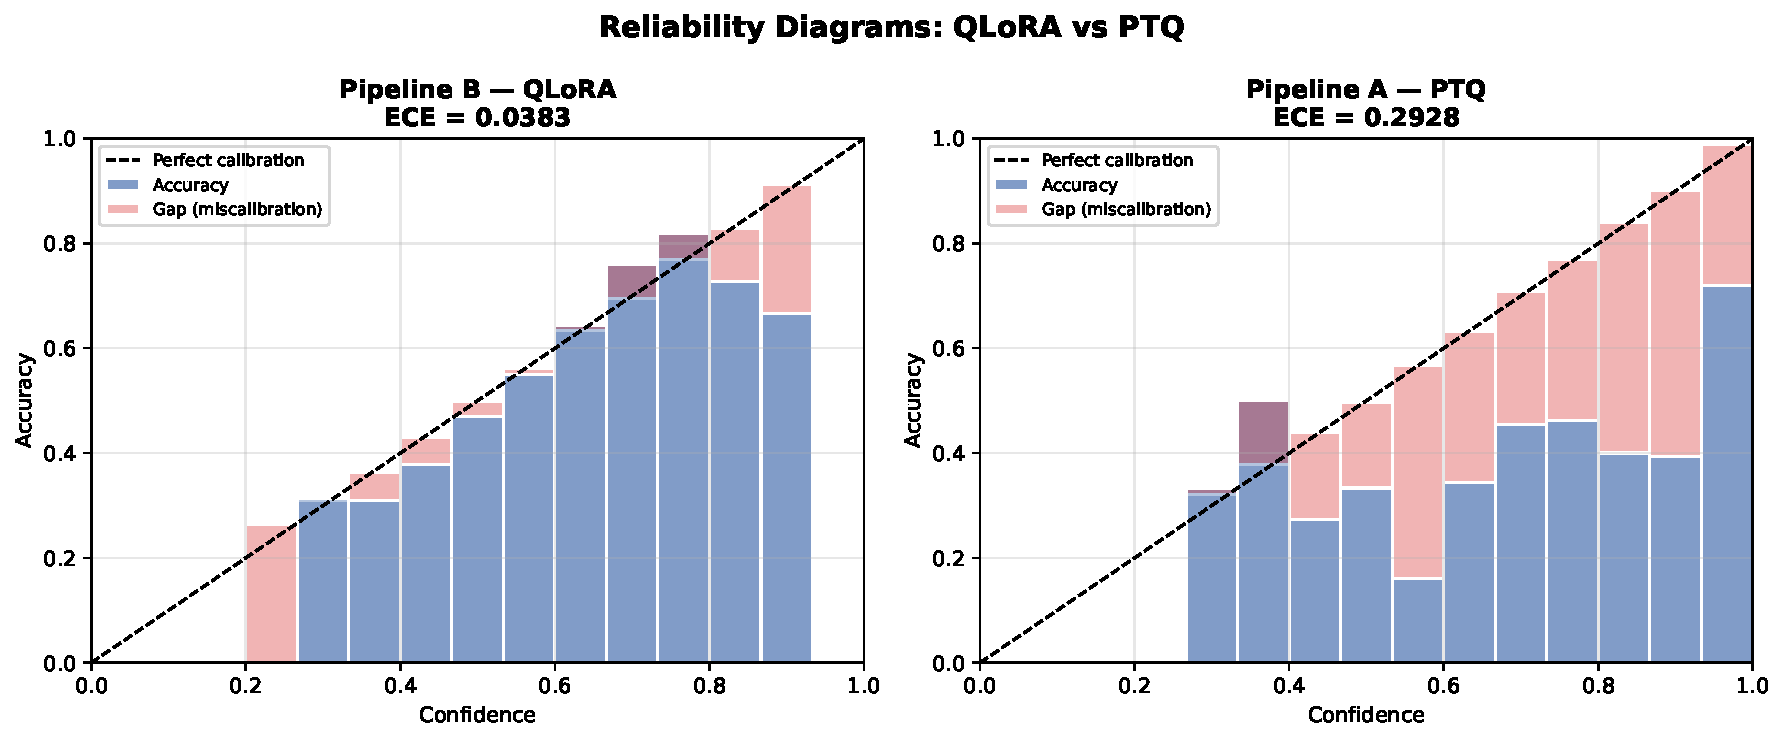
\includegraphics[width=\linewidth]{fig1_reliability_diagrams.pdf}
\end{center}
\caption{Reliability diagrams for Pipeline B (\qlora) and Pipeline A (\ptq).}
\label{fig:reliability}
\end{figure}

Pipeline A achieves substantially higher task accuracy, 61.2\% versus 38.1\%, reflecting the difference in instruction-tuning quality between a professionally trained model and one fine-tuned on 800 samples. However, across every calibration metric, Pipeline B outperforms Pipeline A substantially.

The most striking finding is the overconfidence rate. Pipeline A is confidently wrong, meaning confidence greater than 0.7 on an incorrect prediction, on 29.7\% of all samples. Pipeline B exhibits this behavior on only 0.9\% of samples, a 33x difference. In absolute terms, this means that for every 100 evaluation questions, Pipeline A expresses high confidence on approximately 30 incorrect predictions.

The mean confidence gap, 0.412 versus 0.904, reveals distinct behavioral profiles. Pipeline B distributes its confidence across a broader range and hedges when uncertain. Pipeline A is nearly always confident: its average confidence is 0.843 even on incorrect predictions, with only a small gap relative to correct predictions. This suggests that, in this setup, the model has limited ability to distinguish between correct and incorrect predictions using its own answer-choice probabilities.

\subsection{Per-dataset results}

Table~\ref{tab:dataset-results} and Figure~\ref{fig:per-dataset} present per-dataset breakdowns. The calibration gap is consistent across all three benchmarks, reducing the likelihood that the aggregate result is driven by a single dataset-specific artifact.

\begin{table}[t]
\caption{Per-dataset calibration results.}
\label{tab:dataset-results}
\begin{center}
\begin{tabular}{lllllll}
\toprule
Dataset & B \ece{} & A \ece{} & B overconf. & A overconf. & B acc. & A acc. \\
\midrule
MMLU & 0.05 & 0.36 & 0.01 & 0.34 & 0.37 & 0.51 \\
ARC-Challenge & 0.09 & 0.21 & 0.00 & 0.21 & 0.51 & 0.75 \\
TruthfulQA & 0.16 & 0.33 & 0.02 & 0.33 & 0.26 & 0.58 \\
\bottomrule
\end{tabular}
\end{center}
\end{table}

\begin{figure}[t]
\begin{center}
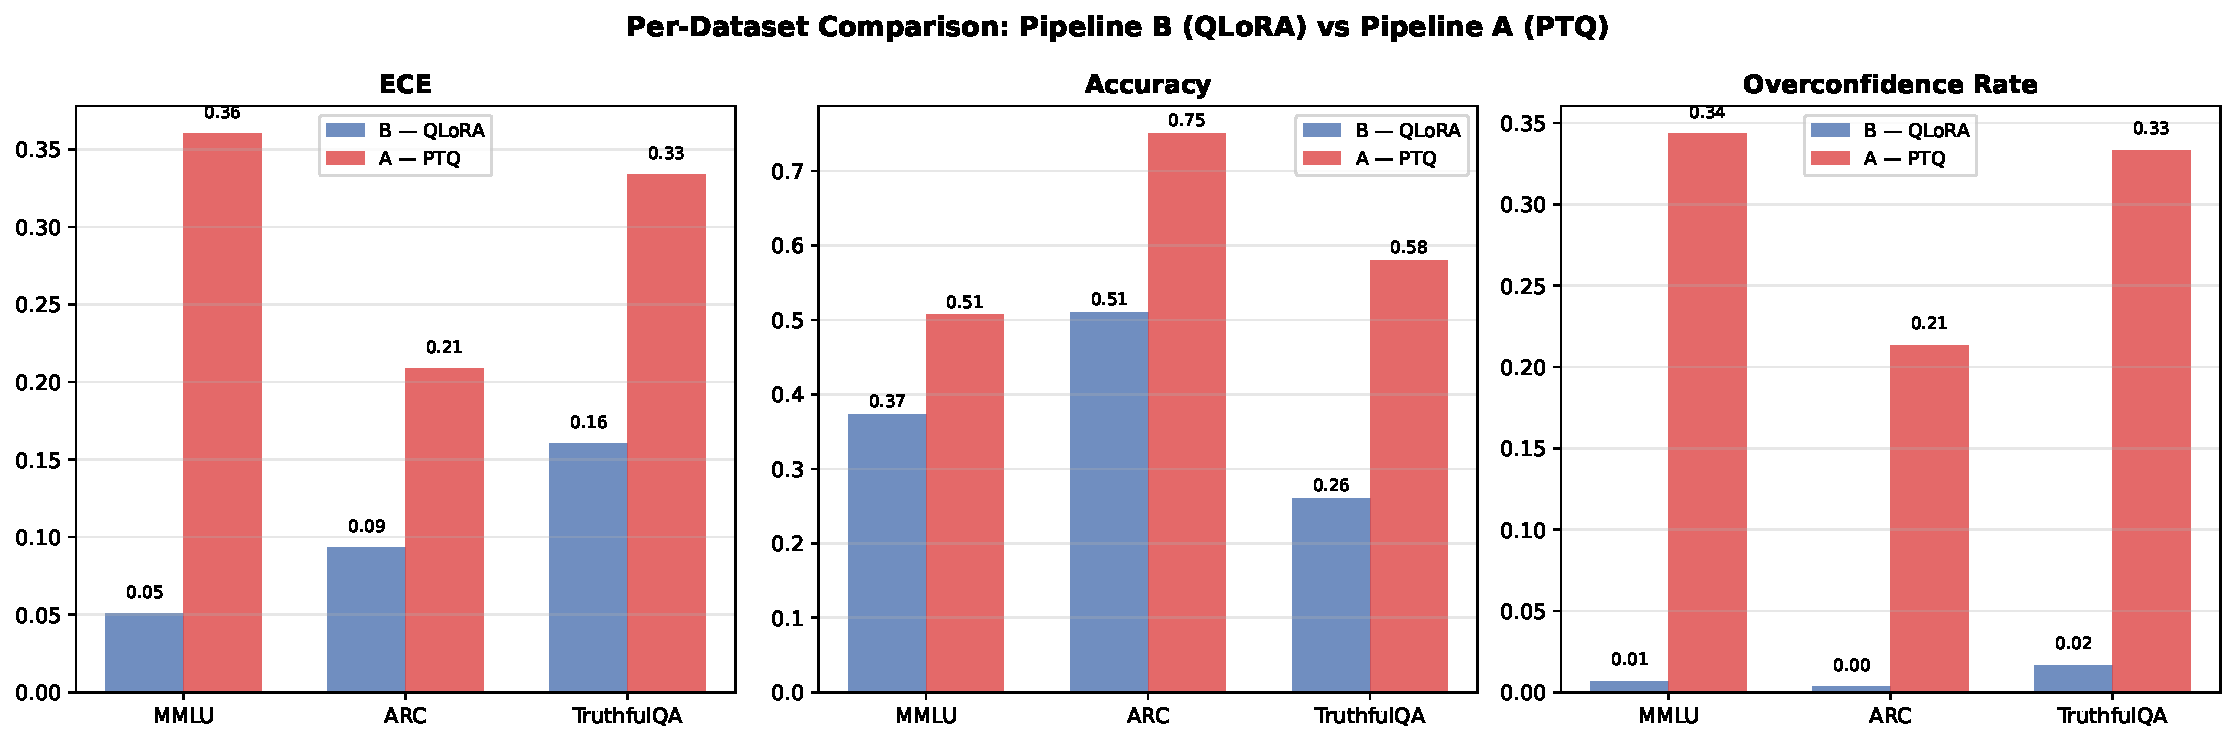
\includegraphics[width=\linewidth]{fig3_per_dataset_comparison.pdf}
\end{center}
\caption{Comparative performance across MMLU, ARC-Challenge, and TruthfulQA.}
\label{fig:per-dataset}
\end{figure}

TruthfulQA shows the most safety-relevant effect. Pipeline A achieves 58\% accuracy on a dataset designed to elicit plausible false statements, yet exhibits an \ece{} of 0.33 and a 33\% overconfidence rate. This means that for approximately every three questions Pipeline A answers incorrectly on TruthfulQA, it expresses high confidence on one of them.

ARC-Challenge is notable for Pipeline B's zero overconfidence rate. Despite the increased difficulty of multi-step reasoning questions, the \qlora{} model never assigns high confidence to a wrong answer in this sample. This extreme conservatism is consistent with the undertraining hypothesis discussed in Section~\ref{sec:discussion}.

\subsection{Calibration-accuracy tradeoff}

Figure~\ref{fig:delta} plots the difference in accuracy against the difference in \ece{} for each dataset, where the difference is computed as Pipeline A minus Pipeline B. All three datasets fall in the top-right quadrant: Pipeline A gains accuracy at the cost of \ece. The pattern holds across all evaluated datasets, suggesting a systematic tradeoff rather than a dataset-specific result.

\begin{figure}[t]
\begin{center}
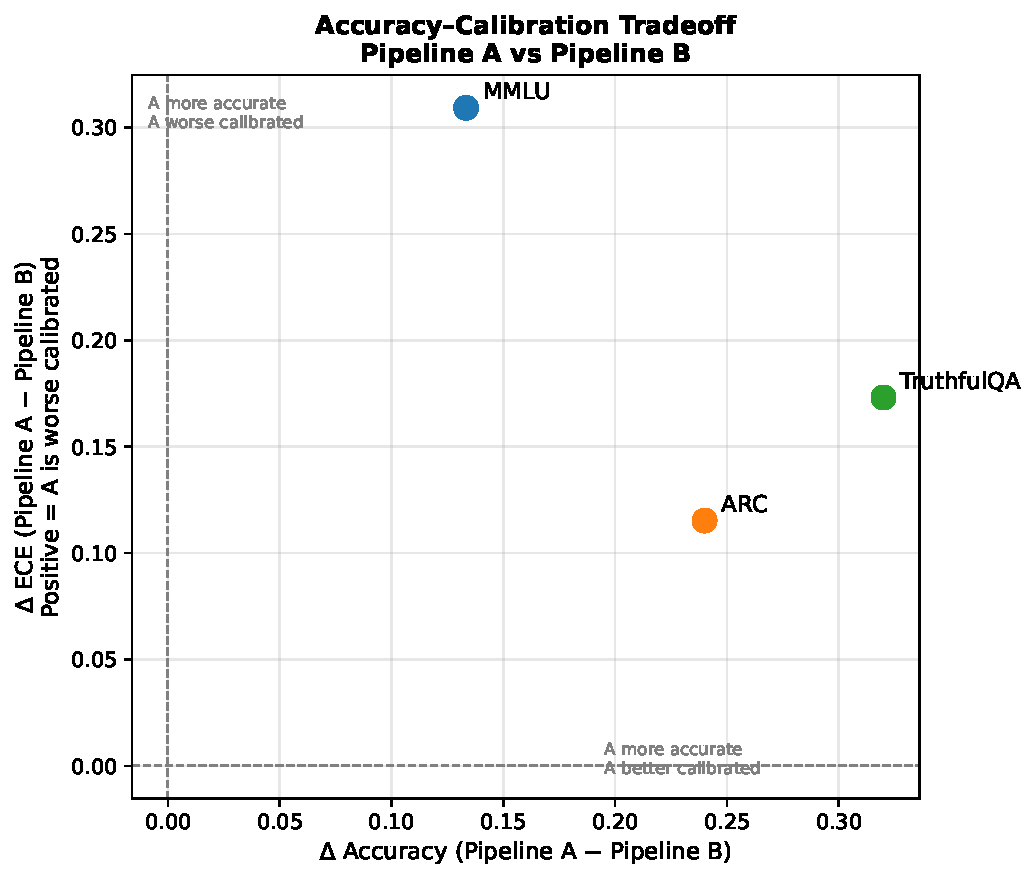
\includegraphics[width=0.78\linewidth]{fig4_delta_accuracy_vs_ece.pdf}
\end{center}
\caption{Difference in accuracy versus difference in \ece{} for each dataset, computed as Pipeline A minus Pipeline B.}
\label{fig:delta}
\end{figure}

This tradeoff has direct implications for deployment decisions. An engineer choosing between pipelines based solely on accuracy metrics would select Pipeline A. Our results show that this choice comes with a hidden cost: less reliable calibration about model uncertainty.

\section{Discussion}
\label{sec:discussion}

\subsection{The undertraining-as-regularization hypothesis}

Why does Pipeline B exhibit dramatically better calibration despite lower accuracy? A plausible explanation is an undertraining-as-regularization effect: a model fine-tuned on 800 samples does not develop the assertive, high-confidence response patterns of a model trained on far larger instruction datasets. The limited training signal is insufficient to push the model toward confident outputs, resulting in distributional hedging behavior that happens to coincide with good calibration.

This is visible in Figure~\ref{fig:confidence}: Pipeline B's confidence distribution is spread across low-to-moderate confidence values for both correct and incorrect predictions, with mean confidence of 0.412. Pipeline A's distribution is concentrated near 1.0, with the correct and incorrect distributions much less separated.

\begin{figure}[t]
\begin{center}
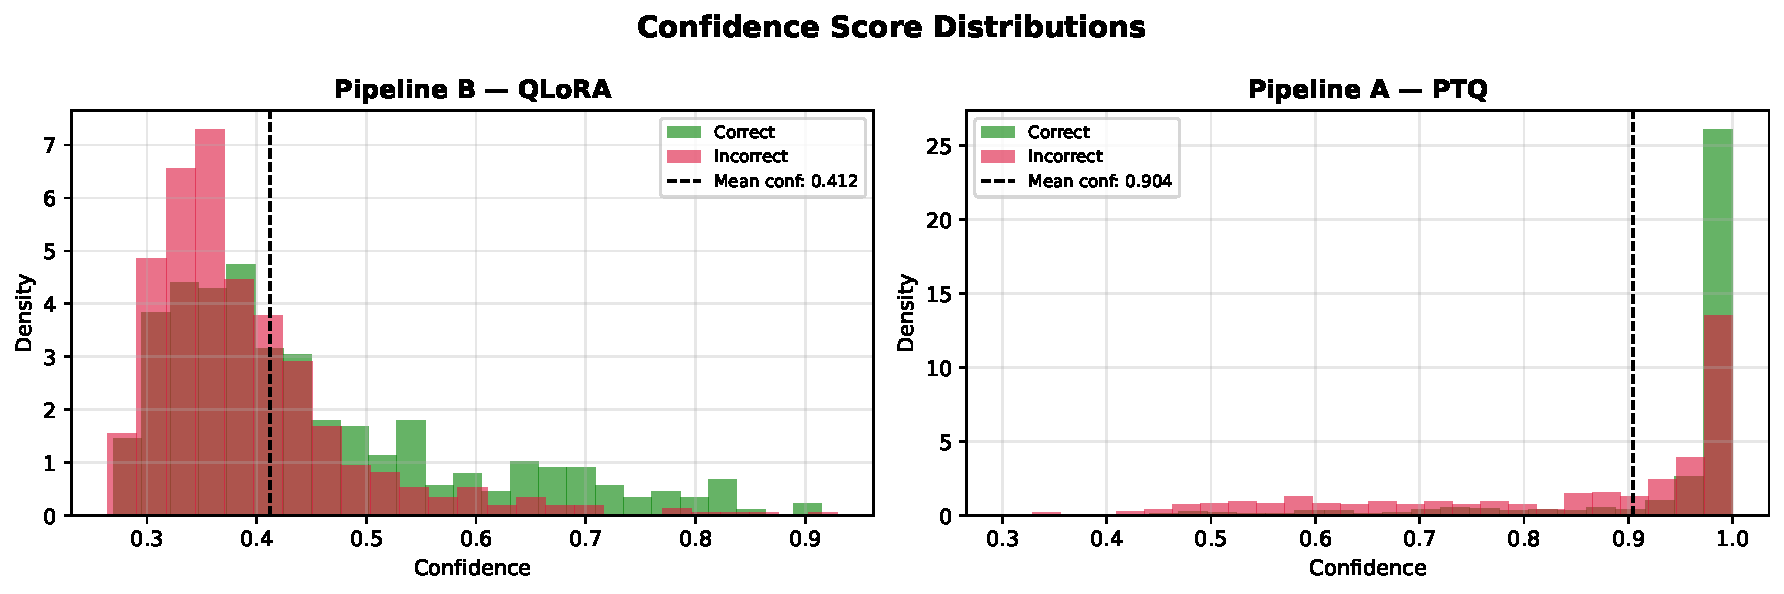
\includegraphics[width=\linewidth]{fig2_confidence_distributions.pdf}
\end{center}
\caption{Confidence distributions for both pipelines.}
\label{fig:confidence}
\end{figure}

The evaluated \ptq{} model appears to have learned to be confident, but not to be accurate about when it is confident. Importantly, this means Pipeline B's good calibration may be a side effect of undertraining rather than an intrinsic property of the \qlora{} quantization order. A \qlora{} model trained on the full Alpaca dataset or on professionally curated instruction data might exhibit calibration profiles closer to Pipeline A. We consider this an important open question.

\subsection{Safety implications}

The practical implication is direct: the \ptq{} deployment pipeline, as it is currently practiced in this setup, using a professionally instruction-tuned model with post-hoc quantization, is associated with models that exhibit systematically higher overconfidence. In agentic settings where downstream components consume model confidence scores for decision thresholds, routing decisions, or human escalation logic, a model with 29.7\% overconfidence rate represents a meaningful safety risk.

TruthfulQA is particularly relevant here. The 33\% overconfidence rate on questions specifically designed to expose models' tendency to produce plausible incorrect information means that Pipeline A will, at nontrivial frequency, assert incorrect answers with high confidence. This is the worst-case calibration failure for deployed language models.

Pipeline B's primary failure mode, underconfidence at 28\%, is less dangerous in many operational contexts. A model that is correct but uncertain prompts appropriate human review. A model that is wrong but certain may not.

\subsection{Implications for deployment practice}

Our results suggest that the choice between \ptq{} and \qlora{} should incorporate calibration as an explicit criterion alongside accuracy and latency. When deployment context requires reliable uncertainty quantification, such as medical question answering, legal research assistance, or autonomous agents, the calibration gap documented here may outweigh the accuracy advantage of \ptq.

A practical mitigation for \ptq{} deployment is post-hoc calibration via temperature scaling. \citet{guo2017calibration} demonstrated that temperature scaling can reduce \ece{} with minimal accuracy impact. Future work should examine whether temperature scaling can close the 7.7x \ece{} gap observed here.

\section{Limitations}
\label{sec:limitations}

We identify three limitations that qualify causal interpretation but do not affect the validity of the empirical comparison.

\paragraph{Instruction-tuning confound.}
The most significant limitation is that pipeline choice is confounded with instruction-tuning scale. Pipeline A uses a professionally tuned model, likely trained on millions of instruction pairs, while Pipeline B uses 800 Alpaca samples. The calibration difference may reflect instruction-tuning data scale rather than quantization order per se. A controlled ablation, fine-tuning the same base model on the same data via both full-precision SFT followed by \ptq{} and quantized \qlora{} fine-tuning, would isolate quantization order as the independent variable but requires additional compute.

\paragraph{Prompt-format asymmetry.}
Pipeline A uses Gemma's chat template; Pipeline B uses the Alpaca instruction format. While each format is appropriate for the respective model's training regime, this introduces a secondary variable. A study using identical prompt formats would provide a cleaner comparison.

\paragraph{Sample size.}
We evaluate on 300 samples per dataset, sufficient for initial \ece{} estimation with 15 bins but small relative to full benchmark evaluation. Larger evaluation sets may reveal dataset-specific variance not captured here. We use 15 bins rather than the standard 10 to improve bin resolution given our sample size of 300 per dataset.

\section{Conclusion}

We presented an empirical comparison of confidence calibration in two real-world LLM deployment pipelines: post-training quantization and \qlora-based fine-tuning. Using Gemma-2-2B as the base model family and evaluating across MMLU, ARC-Challenge, and TruthfulQA, we found that the evaluated \ptq{} pipeline configuration exhibits a 7.7x higher Expected Calibration Error and a 33x higher overconfidence rate than the \qlora{} pipeline, despite achieving 23 percentage points higher task accuracy.

The central finding is simple: accuracy and calibration are not jointly optimized by current deployment practices. The pipeline that yields higher accuracy also exhibits substantially higher overconfidence. For production systems where calibration safety matters, such as agents, medical applications, and high-stakes decision support, this tradeoff is nontrivial and currently invisible to standard evaluation practice.

We propose that calibration metrics, particularly overconfidence rate, should become standard components of LLM deployment evaluation alongside accuracy and latency. The 4-bit quantized models that dominate edge deployment deserve the same calibration scrutiny as their full-precision counterparts. Ignoring calibration in deployment is not a neutral choice; it implicitly accepts overconfident behavior.

\bibliography{main}
\bibliographystyle{tmlr}

\appendix
\section{Reproducibility Notes}

The experiments use 300 examples per benchmark with seed 42. Pipeline A is evaluated with Gemma's native chat template, while Pipeline B is evaluated with the Alpaca instruction format used during its fine-tuning. Confidence is extracted by normalizing logits over the answer tokens A, B, C, and D at the final prompt position.

\end{document}
